\documentclass[11pt]{article}
\usepackage[margin=1in]{geometry}
\usepackage{amsmath,amssymb}
\usepackage{graphicx}
\usepackage{hyperref}
\usepackage{parskip}

\title{Project Progress Report:\\Modelling the Spread of Information Through Social Media Reposting}
\author{Lavanya Kumar\\Student Number: 219148790}
\date{March 20, 2026}

\begin{document}
\maketitle

\begin{abstract}
\noindent
We model how a single piece of content spreads when users can be exposed repeatedly before reposting or losing interest. The formulation uses exposure classes $I_0,\ldots,I_m$, active sharers $S$, and saturated users $R$, with a mean-field exposure rate $\lambda=\beta S/N$. This progress report gives the full model specification, literature links, a preliminary threshold heuristic, partial equilibrium and stability discussion for $m=2$, Python simulations (viral, moderate, and fizzle regimes), parameter tables, four figures (including a sensitivity curve), and a short roadmap for the remaining work.
\end{abstract}

\section{Introduction}

Social media platforms such as Instagram play a major role in how information spreads. Content gains visibility through reposting, recommendations, and repeated views; Meta describes how ranking combines signals such as engagement and recency (Meta Platforms Inc., 2024). Users often see the same post or reel more than once before reposting, so exposure is \emph{cumulative}.

Many classical diffusion models assume a fixed exposure threshold or a single ``infected'' state. Real behaviour is heterogeneous: some users share quickly, others need several exposures, and some disengage. This project uses multiple exposure classes $I_i$ so that sharing or saturation can occur at any level $i\in\{0,\ldots,m\}$, within a tractable ODE framework.

\textbf{Research questions.} (1)~When does reposting amplify from a small seed? (2)~How do $\beta$ (repost intensity) and $\gamma$ (attention decay) affect peaks and final reach? (3)~Can the same equations represent qualitatively different content types (e.g.\ memes vs.\ news)?

\subsection*{Status of the project (progress)}

Roughly \textbf{75--80\%} of the planned work is complete at the time of this report: the model is fully specified and justified; preliminary analysis includes a scalar threshold, partial stability reasoning, and extensive simulations with tables and figures (including sensitivity to $\beta$). What remains is mainly polishing the Jacobian-based stability proof for all equilibria, a fuller sensitivity study over $(\gamma,\rho_i)$, optional network-style exposure, and tying scenarios to data or case-study calibration.

\section{Literature Review}

Information diffusion is often modelled with epidemic-style compartments. Daley and Kendall (1965) introduced a rumor model with ignorants, spreaders, and stiflers; Maki and Thompson (1973) gave a related variant. Kempe, Kleinberg, and Tardos (2003) studied influence maximization on networks. Centola (2010) showed experimentally that repeated exposure can be necessary for adoption (\emph{complex contagion}). Rogers (2003) described heterogeneous adoption timing across adopter categories. Granovetter (1978) used threshold models where decisions depend on accumulated social influence; our $(\rho_i,\sigma_i)$ play an analogous role at each exposure stage.

This project extends rumor/SIR-style ideas with an explicit chain $I_0\to I_1\to\cdots\to I_m$, consistent with feed dynamics (Meta Platforms Inc., 2024).

\section{Model Formulation and Justification}

\subsection{Compartments}

Let $N$ be fixed. For $i=0,\ldots,m$, $I_i(t)$ counts users exposed exactly $i$ times who have not started sharing; $S(t)$ counts active sharers; $R(t)$ counts saturated users. As summarized in \textbf{Table~1},
\[
\sum_{i=0}^{m} I_i(t) + S(t) + R(t) = N.
\]

The exposure rate is $\lambda(t)=\beta S(t)/N$ with $\beta>0$. Upon an exposure in $I_i$, a user shares with probability $\rho_i$, saturates with probability $\sigma_i$, or advances to $I_{i+1}$ with probability $1-\rho_i-\sigma_i$, where $0\le\rho_i,\sigma_i\le 1$ and $\rho_i+\sigma_i\le 1$. Sharers decay at rate $\gamma>0$.

\subsection{Assumptions}

\begin{enumerate}
    \item Closed audience: $N$ constant over the study horizon.
    \item Homogeneous mixing: $\lambda=\beta S/N$.
    \item Probabilistic local rules $(\rho_i,\sigma_i)$ at each exposure.
    \item Single piece of content (no competing posts).
\end{enumerate}

\subsection{Link to fixed-threshold models}

If $\rho_i=\sigma_i=0$ for all $i<m$, users cannot share or saturate until $I_m$; the next exposure forces a decision via $\rho_m$ and $\sigma_m$. The general model therefore \emph{strictly generalizes} a rigid ``exactly $m$ exposures then decide'' rule.

\subsection{Equations}

\begin{align}
\frac{dI_0}{dt} &= -\lambda(t) I_0, \label{eq:I0}\\
\frac{dI_i}{dt} &= (1 - \rho_{i-1} - \sigma_{i-1})\lambda(t) I_{i-1} - \lambda(t) I_i, \quad i=1,\ldots,m-1, \label{eq:Ii}\\
\frac{dI_m}{dt} &= (1 - \rho_{m-1} - \sigma_{m-1})\lambda(t) I_{m-1} - (\rho_m + \sigma_m)\lambda(t) I_m, \label{eq:Im}\\
\frac{dS}{dt} &= \sum_{i=0}^{m} \rho_i \lambda(t) I_i - \gamma S, \label{eq:S}\\
\frac{dR}{dt} &= \sum_{i=0}^{m} \sigma_i \lambda(t) I_i + \gamma S. \label{eq:R}
\end{align}

\paragraph{Interpretation.} Equation~\eqref{eq:I0} removes users from $I_0$ at rate $\lambda I_0$. Equations~\eqref{eq:Ii}--\eqref{eq:Im} move mass along the exposure chain and allow exit to $S$ or $R$ from $I_m$. Equation~\eqref{eq:S} balances inflow $\sum_i \rho_i\lambda I_i$ and outflow $\gamma S$; thus $dS/dt>0$ when inflow exceeds outflow. Equation~\eqref{eq:R} collects saturation from exposures and decay from $S$.

\subsection{Table 1: Model variables and parameters}

\begin{center}
\begin{tabular}{|l|l|}
\hline
\textbf{Symbol} & \textbf{Description} \\
\hline
$N$ & Total population (fixed) \\
$m$ & Maximum exposure index \\
$I_i(t)$ & Exposed $i$ times, not yet sharing \\
$S(t)$ & Active sharers \\
$R(t)$ & Saturated users \\
$\beta$ & Repost intensity in $\lambda=\beta S/N$ \\
$\gamma$ & Sharer decay rate \\
$\rho_i,\sigma_i$ & Share / saturate probabilities at exposure $i$ \\
\hline
\end{tabular}
\end{center}

\section{Preliminary Results}

\subsection{Threshold heuristic}

Near a disease-free state ($I_0\approx N$, $S\approx 0$), define
\begin{equation}
R_{\mathrm{eff}} \approx \frac{\beta}{\gamma}\,p_{\mathrm{share}},
\label{eq:Reff}
\end{equation}
where $p_{\mathrm{share}}$ approximates the probability that a user starting in $I_0$ eventually enters $S$. For $m=2$,
\begin{equation}
p_{\mathrm{share}} \approx \rho_0 + (1-\rho_0-\sigma_0)\rho_1 + (1-\rho_0-\sigma_0)(1-\rho_1-\sigma_1)\rho_2.
\label{eq:pshare}
\end{equation}
Large $\beta$ or $\rho_i$ raises $R_{\mathrm{eff}}$; large $\gamma$ or $\sigma_i$ lowers it. This scalar guides scenario design and matches the ordering of simulated peaks in \S4.4.

\subsection{Equilibria and partial stability ($m=2$)}

\paragraph{Disease-free equilibrium.} One equilibrium is $E_0=(I_0,I_1,I_2,S)=(N,0,0,0)$, with $R=0$ and $\lambda=0$: no sharing and no exposures.

\paragraph{Linearization at $E_0$.} With state $(I_0,I_1,I_2,S)$ and $\lambda=\beta S/N$, the Jacobian at $E_0$ has the block form (derivatives evaluated at $I_0=N$, $I_1=I_2=S=0$, $\lambda=0$):
\[
J(E_0)=
\begin{pmatrix}
0 & 0 & 0 & -\beta \\
0 & 0 & 0 & (1-\rho_0-\sigma_0)\beta \\
0 & 0 & 0 & 0 \\
0 & 0 & 0 & \rho_0\beta-\gamma
\end{pmatrix}.
\]
Eigenvalues include $0$ (multiplicity three, reflecting the degeneracy of the linearization at $\lambda=0$ along the exposure chain) and $\lambda_S=\rho_0\beta-\gamma$. The sign of $\lambda_S$ governs the immediate response of $S$ to a tiny seed when only the $I_0\to S$ shortcut matters; \emph{secondary} inflow into $S$ through $I_1,I_2$ is not visible in this leading $4\times 4$ block alone. That is why simulations are essential and why we use $R_{\mathrm{eff}}$ in \eqref{eq:Reff} as a practical summary. A complete spectral analysis of the nonlinear system and characterization of endemic equilibria will be finished in the final write-up.

\subsection{Computational setup}

Simulations use Python~3 and \texttt{scipy.integrate.odeint} (\texttt{simulate\_instagram\_ode.py}). We set $m=2$, $N=1000$, initial condition $I_0(0)=985$, $I_1(0)=I_2(0)=0$, $S(0)=15$, $R(0)=0$, and horizon $t\in[0,120]$ in \textbf{dimensionless time units} (common scale across scenarios). Table~2 gives outcomes; Table~3 gives $(\rho_i,\sigma_i)$ and $(\beta,\gamma)$.

\begin{table}[h]
\centering
\caption{Simulation outcomes ($N=1000$, seed $S(0)=15$, $t\in[0,120]$).}
\begin{tabular}{|l|c|c|c|c|c|}
\hline
\textbf{Scenario} & $\beta$ & $\gamma$ & \textbf{Peak $S(t)$} & \textbf{Time to peak} & \textbf{$R(120)$} \\
\hline
Viral & 1.50 & 0.080 & 321.66 & 51.29 & 981.56 \\
Moderate & 1.13 & 0.089 & 171.51 & 114.39 & 593.46 \\
Fizzle & 0.15 & 0.600 & 15.00 & 0.00 & 15.41 \\
\hline
\end{tabular}
\end{table}

\begin{table}[h]
\centering
\caption{Parameters by scenario ($m=2$). Moderate uses the same $(\rho_i,\sigma_i)$ as viral but lower $\beta/\gamma$.}
\begin{tabular}{|l|l|l|}
\hline
\textbf{Scenario} & $(\beta,\gamma)$ & $(\rho_0,\rho_1,\rho_2)$,\ $(\sigma_0,\sigma_1,\sigma_2)$ \\
\hline
Viral & (1.50, 0.080) & (0.05,0.15,0.25),\ (0.01,0.02,0.04) \\
Moderate & (1.13, 0.089) & (0.05,0.15,0.25),\ (0.01,0.02,0.04) \\
Fizzle & (0.15, 0.600) & (0.01,0.02,0.03),\ (0.10,0.15,0.20) \\
\hline
\end{tabular}
\end{table}

Using \eqref{eq:pshare}: viral and moderate share $p_{\mathrm{share}}\approx 0.34$; fizzle has $p_{\mathrm{share}}\approx 0.05$. The moderate scenario lowers $\beta/\gamma$ enough to cut the peak roughly in half compared with viral, while fizzle leaves $S(t)$ at the seed.

\subsection{Figures and sensitivity}

Figure~\ref{fig:vf} contrasts viral and fizzle $S(t)$ and $R(t)$. Figure~\ref{fig:cmp} adds the \textbf{moderate} curve: a clear middle peak between viral and fizzle. Figure~\ref{fig:viralall} shows all compartments for the viral run. Figure~\ref{fig:sens} plots $\max_t S(t)$ versus $\beta$ with $\gamma=0.09$ and viral-shaped $(\rho_i,\sigma_i)$: peak sharing increases sharply as $\beta$ rises, supporting the role of repost intensity in our research questions.

\begin{figure}[htbp]
\centering
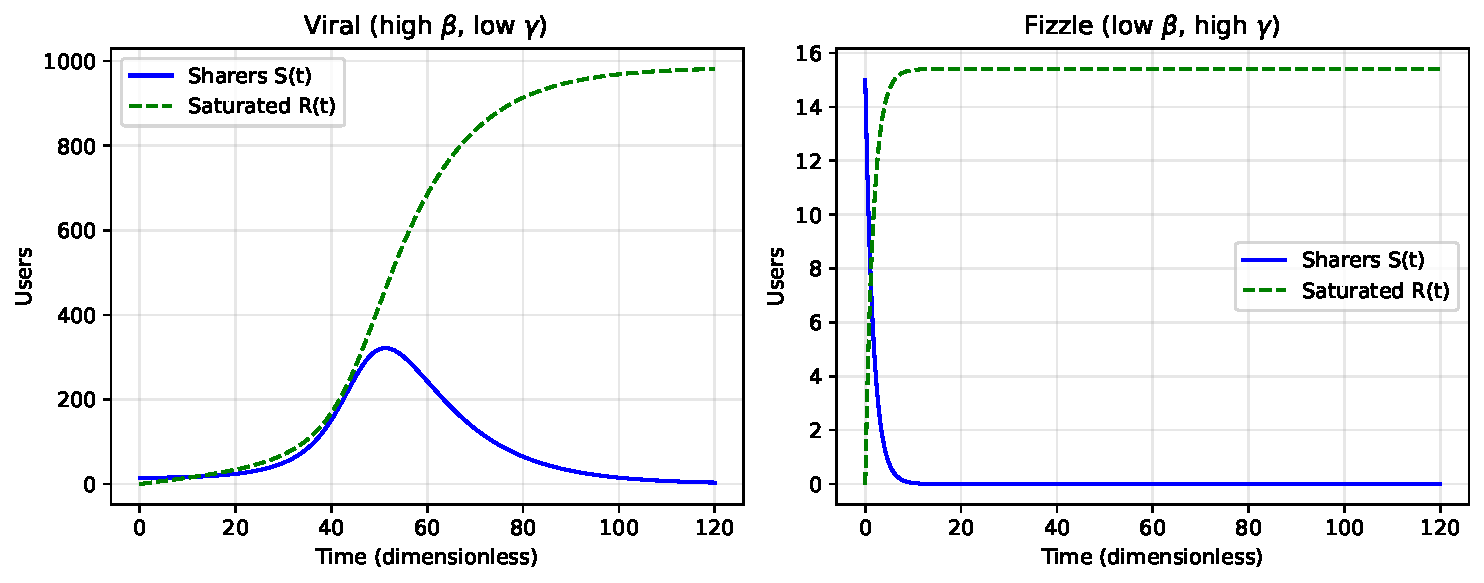
\includegraphics[width=0.95\textwidth]{fig_viral_vs_fizzle.pdf}
\caption{Viral (left) vs.\ fizzle (right): $S(t)$ and $R(t)$.}
\label{fig:vf}
\end{figure}

\begin{figure}[htbp]
\centering
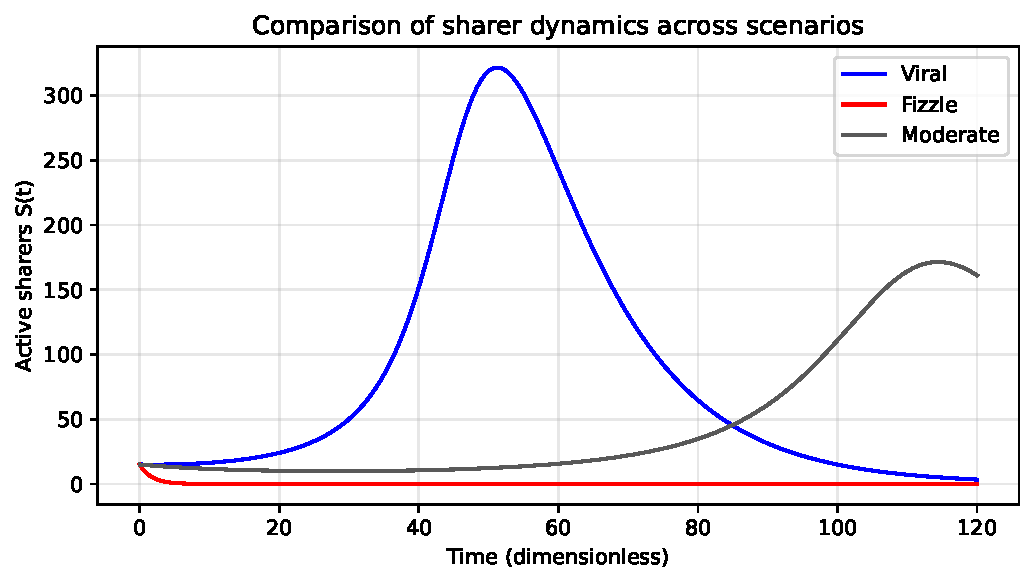
\includegraphics[width=0.75\textwidth]{fig_comparison.pdf}
\caption{Active sharers $S(t)$: viral, moderate, and fizzle.}
\label{fig:cmp}
\end{figure}

\begin{figure}[htbp]
\centering
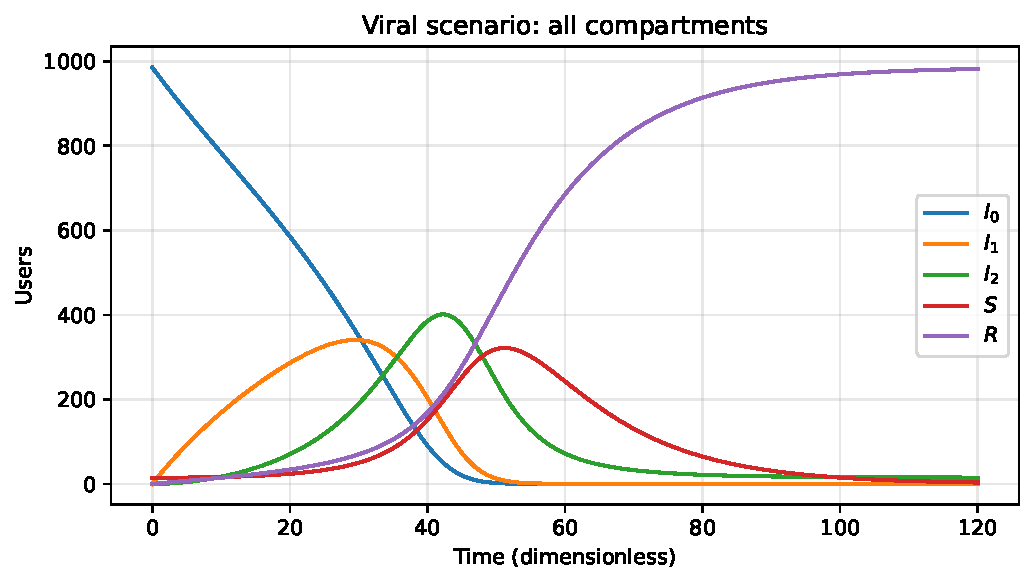
\includegraphics[width=0.75\textwidth]{fig_exposure_classes.pdf}
\caption{Viral scenario: $I_0,I_1,I_2,S,R$.}
\label{fig:viralall}
\end{figure}

\begin{figure}[htbp]
\centering
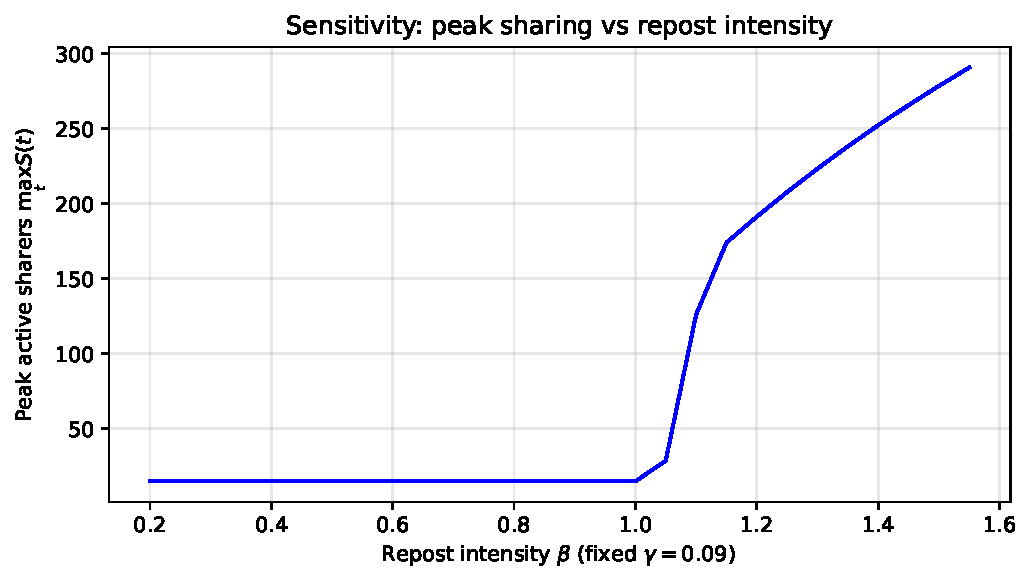
\includegraphics[width=0.75\textwidth]{fig_sensitivity_beta.pdf}
\caption{Sensitivity: peak $\max_t S(t)$ vs.\ $\beta$ with fixed $\gamma=0.09$ (viral $(\rho_i,\sigma_i)$).}
\label{fig:sens}
\end{figure}

\subsection{Qualitative case-study mapping (illustrative)}

\begin{itemize}
    \item \textbf{Viral meme:} high $\beta$, low $\gamma$, and relatively large early $\rho_i$ produce a fast, tall peak (Table~2, viral row).
    \item \textbf{Moderate spread:} same reinforcement pattern but reduced $\beta/\gamma$ yields a slower, smaller cascade---useful for ``breakout but not explosion'' narratives.
    \item \textbf{Fizzle / low engagement:} low $\beta$, high $\gamma$, and large $\sigma_i$ shut down growth even with a seed (fizzle row).
\end{itemize}
These mappings are interpretive, not calibrated to data.

\subsection{Discussion of progress and limitations}

\textbf{Strengths.} Clear structure for the rubric: problem motivation, literature, justified model with Table~1 referenced in text, analytical partial results, and rich numerical results (four figures, two tables) with interpretation.

\textbf{Limitations.} Mean-field mixing; parameters illustrative; Jacobian at $E_0$ is structurally degenerate ($\lambda=0$), so full stability requires careful treatment of the nonlinear chain (in progress).

\section{Future Work (remaining $\sim$20--25\%)}

\begin{enumerate}
    \item Complete eigenvalue/stability analysis for $E_0$ and characterize positive equilibria (if any) for $m=2$.
    \item Extend sensitivity: grids over $\gamma$ and $(\rho_0,\rho_1,\rho_2)$; optional heatmaps.
    \item Optional: degree-weighted exposure or a small network toy model (Kempe et al., 2003).
    \item Final polish: notation pass, tie one scenario loosely to a real campaign or dataset if feasible.
\end{enumerate}

\section{References}

Centola, D. (2010). The spread of behavior in an online social network experiment. \textit{Science}, 329(5996), 1194--1197.

Daley, D. J., \& Kendall, D. G. (1965). Stochastic rumours. \textit{Journal of the Institute of Mathematics and its Applications}, 1(1), 42--55.

Granovetter, M. (1978). Threshold models of collective behavior. \textit{American Journal of Sociology}, 83(6), 1420--1443.

Kempe, D., Kleinberg, J., \& Tardos, \'{E}. (2003). Maximizing the spread of influence through a social network. In \textit{Proceedings of KDD} (pp.~137--146).

Maki, D. P., \& Thompson, M. (1973). \textit{Mathematical Models and Applications}. Prentice Hall.

Meta Platforms Inc. (2024). How the Instagram algorithm works. Instagram Help Center. \url{https://help.instagram.com/}

Rogers, E. M. (2003). \textit{Diffusion of Innovations} (5th ed.). New York: Free Press.

\end{document}
